\subsection{XOR en OR}
De verschillen tussen het leren van de XOR en OR operaties worden hier onderzocht. Het enige verschil tussen de twee operaties is dat XOR gemiddeld 0.5 kans heeft dat het antwoord 1 of 0 is. OR heeft gemiddeld 0.75 kans dat het antwoord een 1 is en 0.25 kans dat het 0 is.

\begin{table}[ht]
    \centering
      $\begin{array}{l || c | c | c | c}
                                    & \text{Aantal verborgen knopen} & \text{XOR} & \text{OR} \\ \hline
        \text{Aantal correct}       & \multirow{2}{*}{4}  & 26 & 47 \\ \cline{1-1} \cline{3-4}
        \text{Percentage \% correct} &                    & 52 & 94 \\ \cline{1-1} \cline{3-4} \hline \hline
        \text{Aantal correct}       & \multirow{2}{*}{8} & 31 & 50 \\ \cline{1-1} \cline{3-4}
        \text{Percentage \% correct} &                    & 62 & 100 \\ \cline{1-1} \cline{3-4} \hline
      \end{array}$
    \caption{Aantal correcte antwoorden over 50 executies met operaties XOR en OR met verschillende aantallen verborgen knopen}
    \label{tab:xoror}
\end{table}

\begin{figure}[ht!]
    \centering
    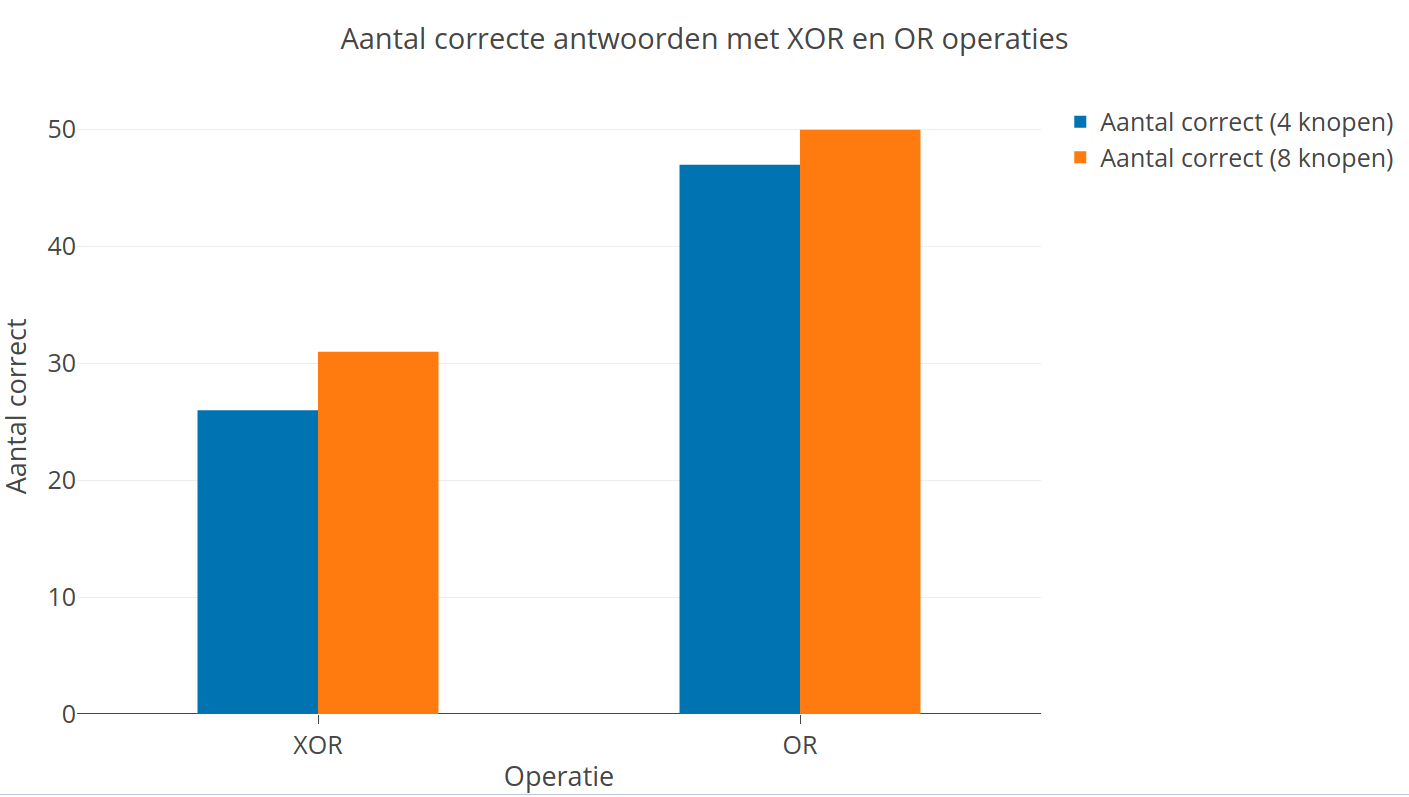
\includegraphics[scale=0.3]{graphs/xoror.png}
    \caption{Grafiek van Tabel \ref{tab:xoror}}
    \label{fig:xoror}
\end{figure}
